\chapter[Experimentos, Análises e Resultados]{Experimentos, Análises e Resultados}
\label{capExperimentos}

Este capítulo fará uma análise baseada em \acs{UX} e \acs{UI} da Plataforma DebugandoED. Este capítulo está organizado da seguinte forma: A seção \ref{secExperimentos} apresentará os detalhes do experimento a ser realizado; A seção \ref{Menu_de_Navegação} apresentará os principais conceitos que serão aplicados aos menus do simulador acima; A seção \ref{Conteúdo_na_Pagina_Inicial} apresentará os principais conceitos que serão aplicados ao conteúdo da página inicial; A seção \ref{Campos_de_Entrada_de_Dados} apresentará os principais conceitos que serão aplicados no conteúdo da página principal; As seções \ref{Formulário de Cadastro} e \ref{Formulário de Login} proporão os conceitos da seção \ref{Campos_de_Entrada_de_Dados} em conjunto no formulário de cadastro e login; A seção \ref{Conteúdo das Telas de Simulação} apresentará os principais conceitos que serão aplicados ao conteúdo da página de simulação ou execução.

%Este capítulo está organizado da seguinte forma: A seção \ref{Menu_de_Navegação} apresenta os principais conceitos que serão aplicados aos menus do simulador acima; A seção \ref{Conteúdo_na_Pagina_Inicial} apresenta os principais conceitos que serão aplicados ao conteúdo da página inicial, como blocos no corpo da página; A seção \ref{Campos_de_Entrada_de_Dados} apresenta os principais conceitos que serão aplicados no conteúdo da página principal, como os bloco no corpo da página; A seção \ref{Formulário de Cadastro} e \ref{Formulário de Login} irá propor os conceitos da seção \ref{Campos_de_Entrada_de_Dados} em conjunto no formulário de cadastro e login; A seção \ref{Conteúdo das Telas de Simulação} apresenta os principais conceitos que serão aplicados ao conteúdo da página de simulação ou execução, como blocos no corpo da página, modais e demais elementos da página.

\section{Experimento}
\label{secExperimentos}

A proposta deste trabalho é aplicar os conceitos e princípios apresentados no \autoref{capFund} à plataforma DebugandoED. Não serão abordadas todas as telas da plataforma, pois algumas delas são, basicamente, os mesmos objetos aplicados a uma nova situação. Serão analisados: menu de navegação, conteúdos da página inicial, campos de entrada de dados, formulário de cadastro, formulário de login e telas de simulação. Para cada um dos itens descritos, a proposta é aplicar o conceito/princípio e propor uma modificação que seja condizente com os mesmos.

\subsection{Base dos Estudos}

A plataforma DebugandoED\footnote{\url{https://debugandoed.facom.ufu.br/}} será utilizada como estudo de caso para a aplicação dos conceitos e princípios apresentados no \autoref{capFund}. Esta plataforma simula estruturas de dados visando abordar os conceitos das estruturas de dados abordados em sala de aula, apresentando de maneira visual e de forma prática as estruturas sem a necessidade do usuário realmente programar a estrutura em questão. A plataforma foi pensada para que não seja necessária a instalação de qualquer software e, com isso, seu acesso é por meio de um navegador web. A tela inicial da plataforma pode ser visualizada na \autoref{debugandoED01}. A plataforma está em constante evolução e está sendo implementada a parte de \textit{gamificação}, com isso, pode ser que algumas telas, com o passar do tempo, possam estar modificadas quando comparadas com as apresentadas neste trabalho.

\begin{figure}[ht]
    \begin{center}
        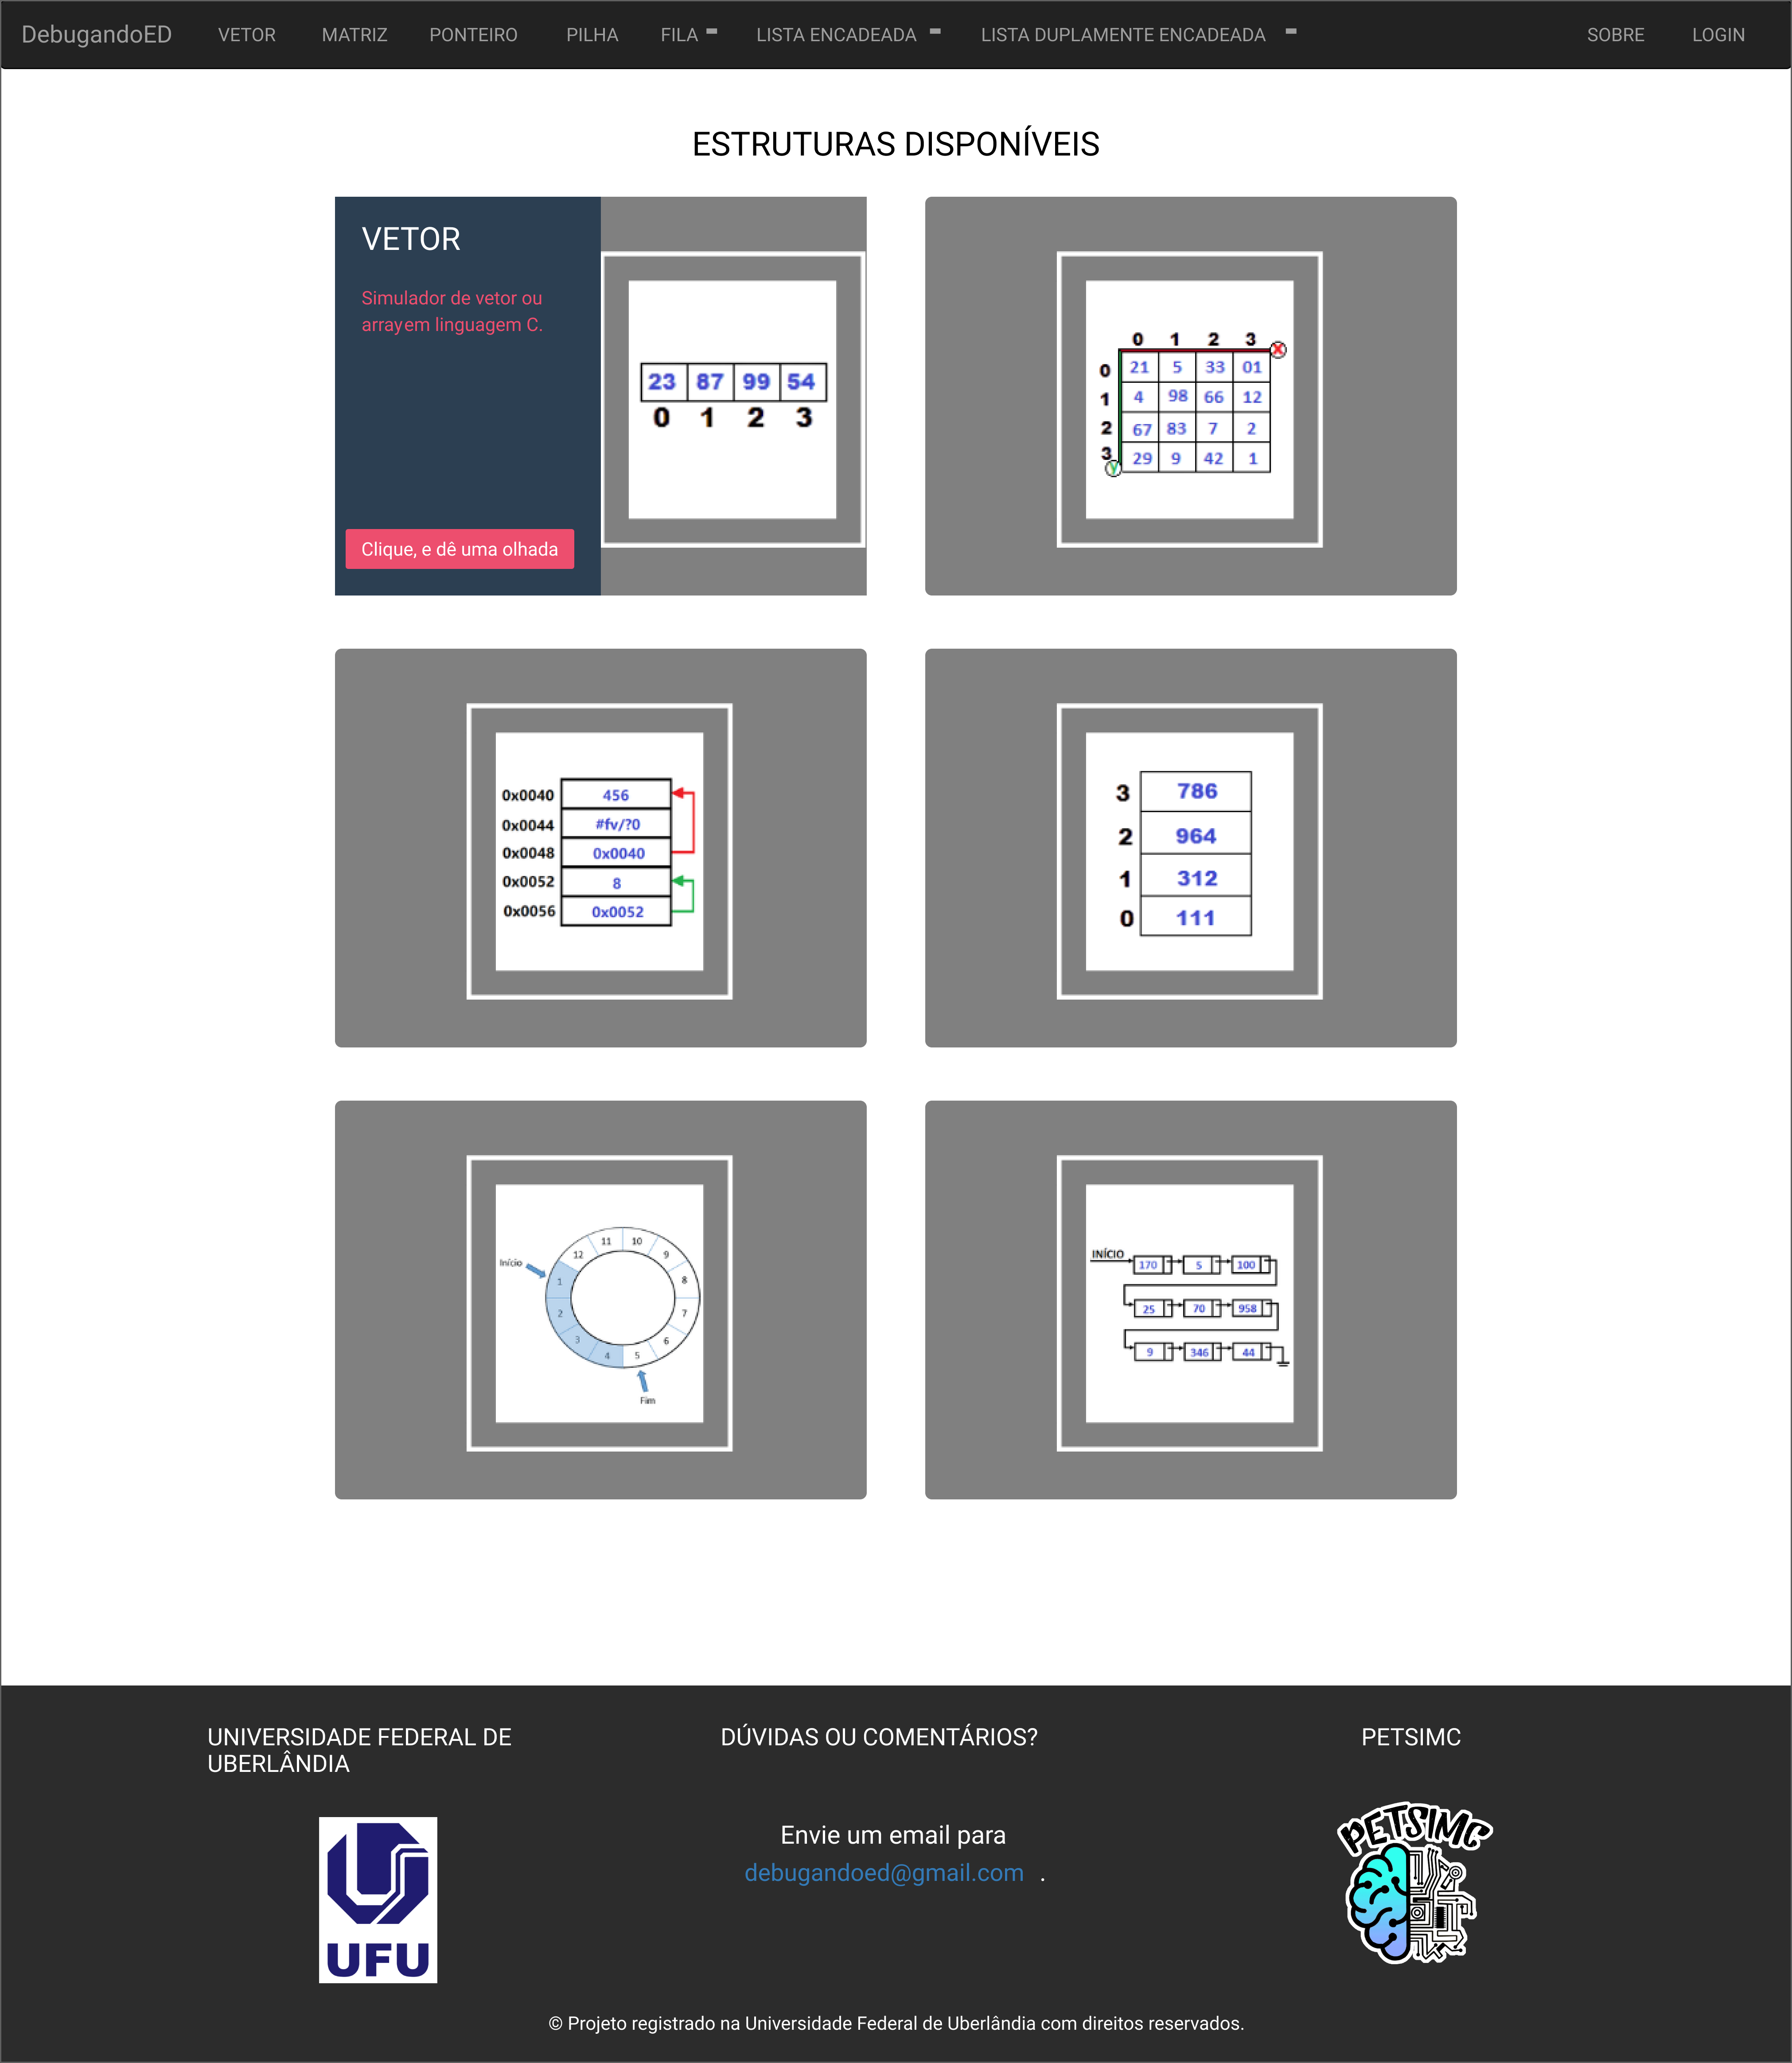
\includegraphics[scale=0.3]{figs/debugandoED01.png}
    \end{center}
    \caption{\label{debugandoED01}Tela inicial da Plataforma DebugandoED.}
    \legend{Fonte: \href{https://debugandoed.facom.ufu.br/}{https://debugandoed.facom.ufu.br}}
\end{figure}


\subsection{Menu de Navegação}
\label{Menu_de_Navegação}

De acordo com o seção de Design de Interfaces (\autoref{Design de Interfaces (UI)}) e a Heurísticas de Estética e Design minimalista de Jakob Nielsen (\autoref{Heurísticas de Jakob Nielsen}), nota-se no menu de opções apresentado na \autoref{debugandoED01}, um desacordo na utilização de cores e contrastes, logo nota-se não haver uma padronização na escala de cores utilizadas.
    
Um simples ajuste de fonte e cor, obtém um contraste melhor e por consequência mais legibilidade, optando-se pelo branco como cor da fonte ao invés do cinza (\autoref{debugandoED-menu} - B) e aumentando o peso da fonte (\autoref{debugandoED-menu} - C).
    
    \begin{figure}[htb]
        \begin{center}
    	    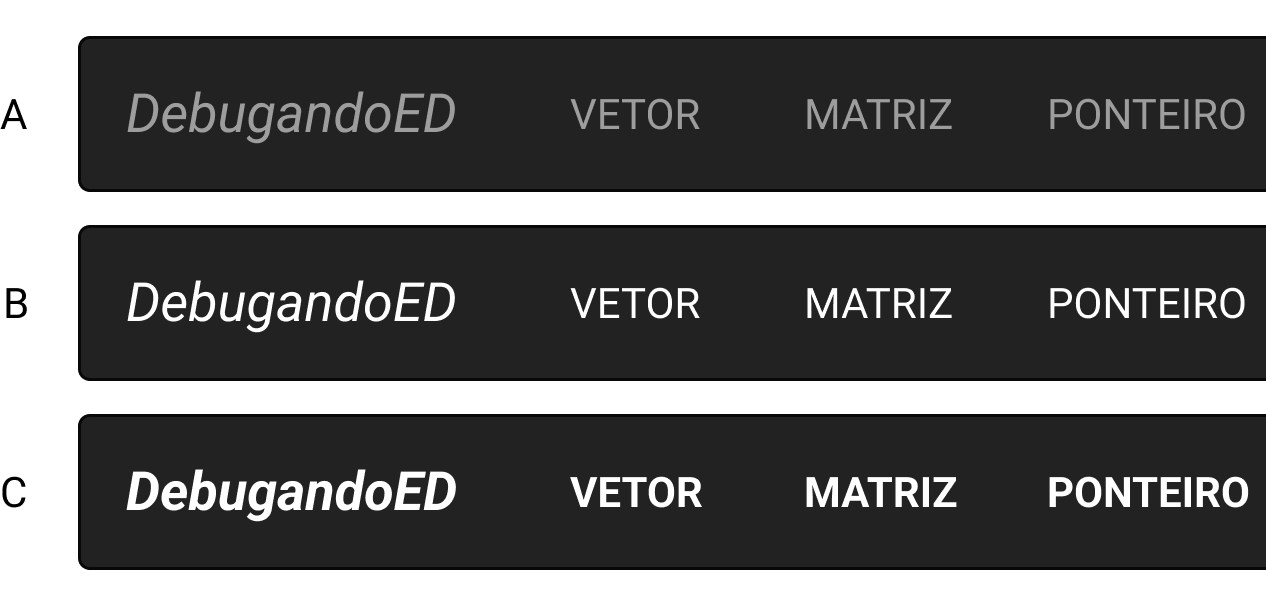
\includegraphics[scale=1]{figs/debugandoED-menu.png}
    	\end{center}
        \caption{\label{debugandoED-menu}Ajustes na fonte do menu: (A) Original; (B) Troca da cor; (C) Aumento do peso da fonte de B.}
    \end{figure}
    
 Outro ponto de Jakob Nielsen, é a heurísticas de reconhecer ao invés de lembrar (\autoref{Heurísticas de Jakob Nielsen}), tornando as abas mais reconhecíveis com ícones, entretanto, em especifico este possui várias abas tornando complexo respeitar o Princípio da Proximidade de Gestalt sendo necessário a utilização de técnicas de responsividade para tela de tamanho diferentes (\autoref{debugandoED-menu-icons}).
 
\begin{figure}[htb]
    \begin{center}
        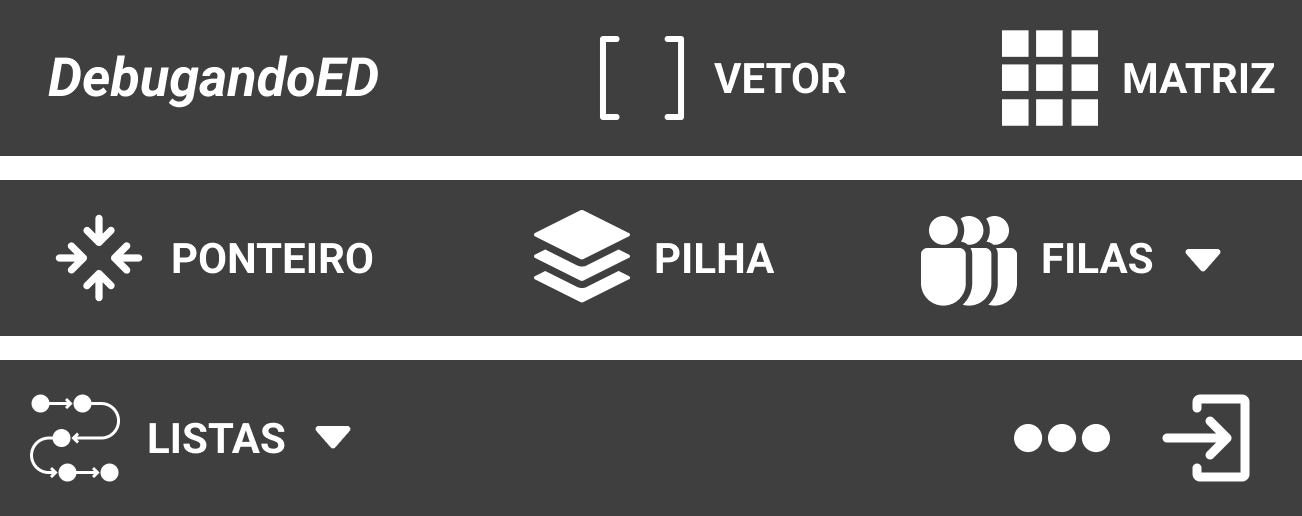
\includegraphics[scale=1]{figs/debugandoED-menu-icons.png}
    \end{center}
    \caption{\label{debugandoED-menu-icons}Proposta de ícones para trabalhar a heurísticas de reconhecer.}
\end{figure}

No conceito da \autoref{Experiência_de_Usuário}, onde é tratado a experiência do usuário, adicionar uma forma visual de localização no menu de navegação na sobreposição do mouse em cima de cada item do menu (\autoref{debugandoED-menu-hovers}), isso apenas localiza o usuário de onde ele está, melhorando sua experiência. A proposta na \autoref{debugandoED-menu-hovers} é um efeito, onde o conteúdo em forma de um botão estivesse se elevando dos demais, logo o destacando.

\begin{figure}[htb]
    \begin{center}
        
\includegraphics[scale=1]{figs/debugandoED-menu-hover.png}
    \end{center}
    \caption{\label{debugandoED-menu-hovers}Exemplo de destaque para localização do item do menu pelo usuário.}
\end{figure}

\subsection{Conteúdo na Página Inicial}
\label{Conteúdo_na_Pagina_Inicial}

De acordo com a correspondência entre o sistema e o mundo real (\autoref{Heurísticas de Jakob Nielsen}), na \autoref{debugandoED-bloco-antes} pode-se notar um dos diversos blocos que a tela inicial possui, com imagens representando outras funcionalidades específicas do sistema, imagens não tão simples para usuário leigos no assunto, embora tenha o efeito de sobreposição do mouse no qual é mostrado mais informações sobre aquele bloco, isto pode ser melhorado colocando alguma forma de indicativo ou informação simplificada sem a necessidade de sobrepor o mouse nos blocos.
    
\begin{figure}[htb]
    \begin{center}
	    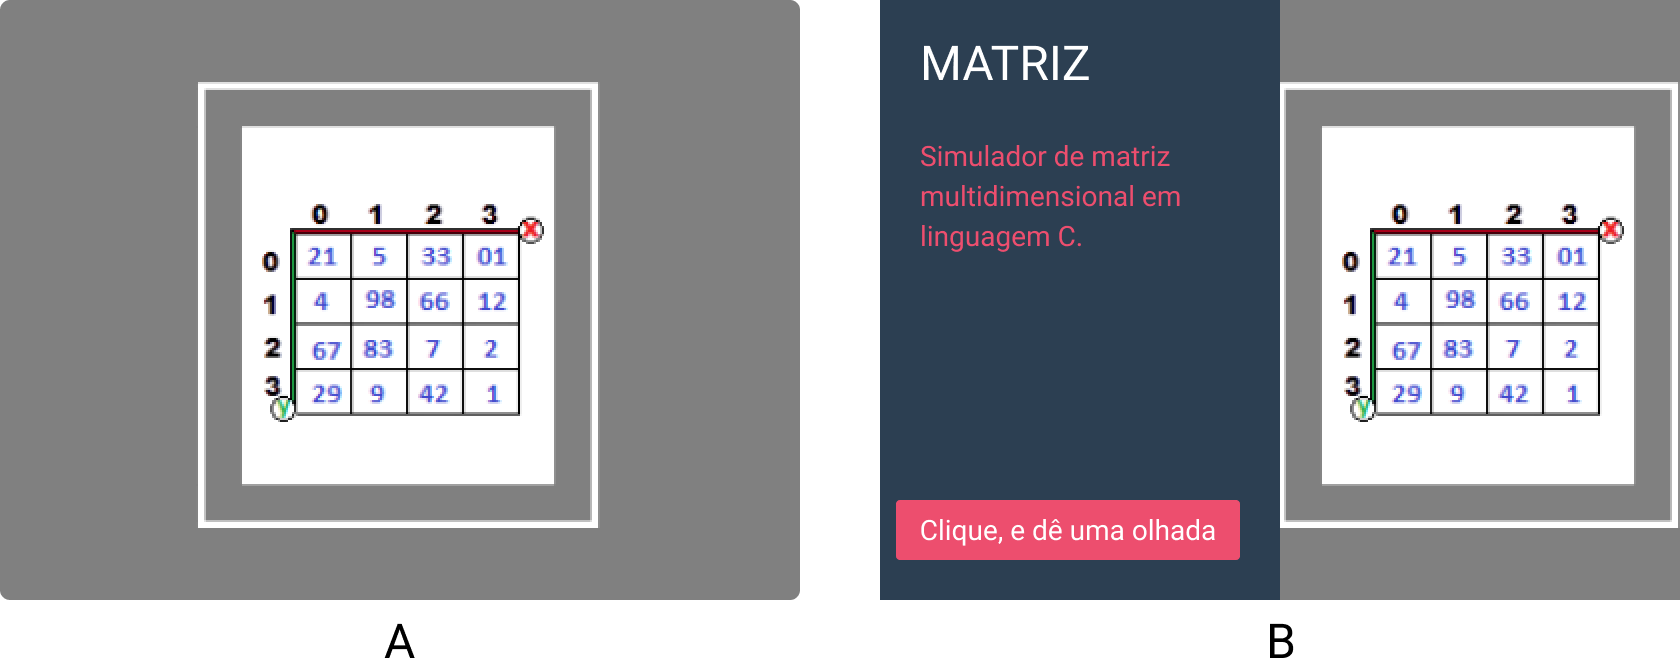
\includegraphics[scale=0.52]{figs/debugandoED-bloco-antes.png}
	\end{center}
    \caption{\label{debugandoED-bloco-antes}Blocos de Matriz (Original): (A) sem sobreposição - (B) com sobreposição.}
\end{figure}
    
\begin{figure}[htb]
    \begin{center}
	    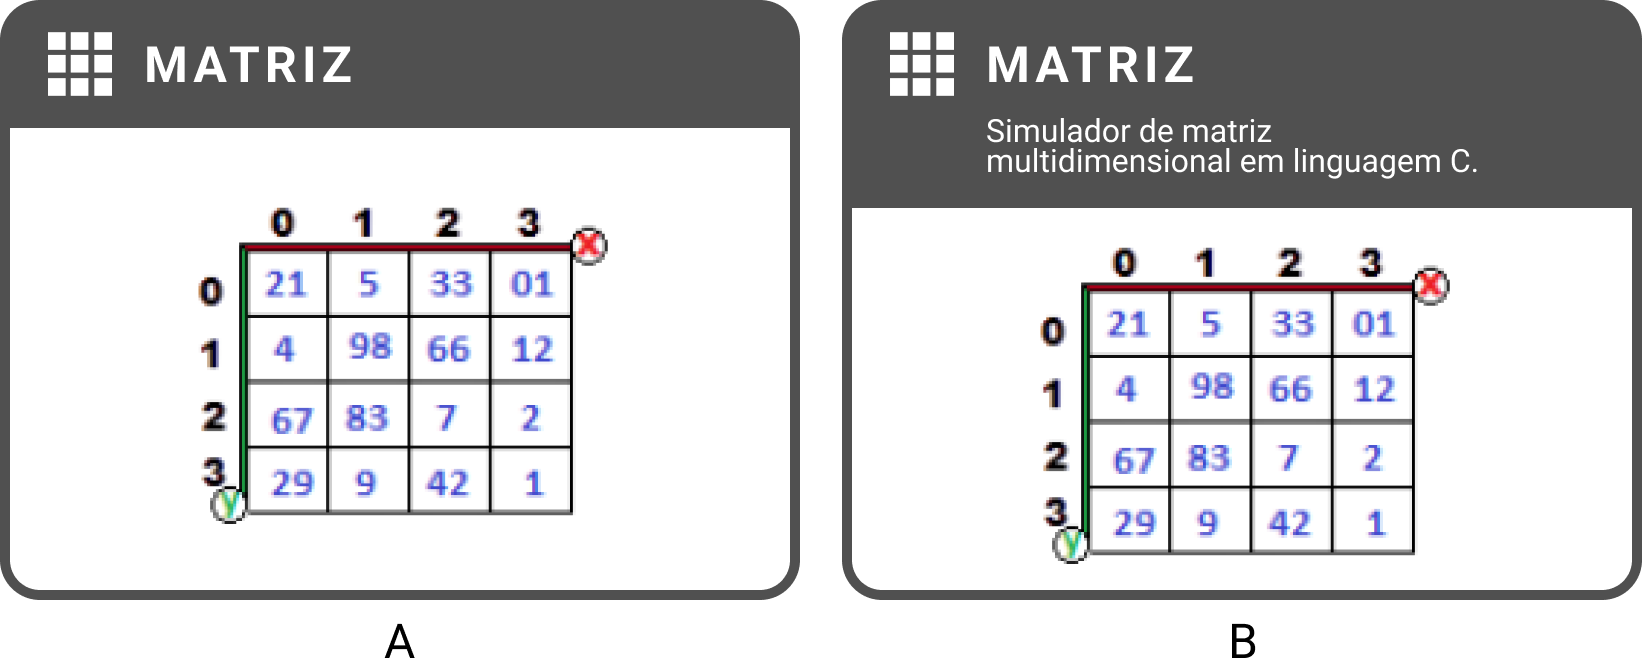
\includegraphics[scale=0.52]{figs/debugandoED-bloco-depois.png}
	\end{center}
        \caption{\label{debugandoED-bloco-depois}Blocos de Matriz (Proposta): (A) sem sobreposição - (B) com sobreposição.}
\end{figure}

Na \autoref{debugandoED-bloco-antes} (A) é apenas uma imagem técnica sobre o bloco, mas como apontando no inicio desta seção, formas mais leigas de identificação são necessárias, não mudando nada para os usuários mais experientes, como na \autoref{debugandoED-bloco-depois} (A), é adicionado o título e o mesmo ícone representativo do menu de navegação, embora não seja obrigatória, proporciona maior acessibilidade e familiaridade aos usuários. 

Na \autoref{debugandoED-bloco-antes} (B), tem-se o efeito de sobreposição do mouse, aqui se repete um desacordo de contraste na utilização das cores e oposição a regra de Flexibilidade e Eficiência da \autoref{Heurísticas de Jakob Nielsen}, no qual o usuário teria de sobrepor o mouse no bloco para assim poder clicar no botão e navegar até a página. Na \autoref{debugandoED-bloco-depois} (B) este botão é removido passando este evento de clique para o bloco em si, não tornando a navegação específica a um botão interno, sendo também mantido o efeito de sobreposição do mouse onde apenas é mostrado uma descrição sobre o conteúdo em si.

Resolvendo também a questão do contraste com a descrição, onde pode ser utilizado uma tonalidade mais escura do próprio bloco e não outra cor, com a fonte na cor branca, criando um contraste nítido e colocando o bloco em cores monocromáticas. As cores em si não são o foco mas sim a disposição do elementos de acordo com a Gestalt, porém tal estudo de cores é de extrema importância para quando se possui um identidade visual definida.

De acordo com o Princípio da Figura-Fundo, para manter o foco nos blocos, cantos arredondados e um contorno, além de estético também servem para fazer embalagens de conteúdo (\autoref{debugandoED-bloco-antes-depois-01} (B)), isto porque os cantos arredondados estão apontados para a parte interna em direção ao centro do retângulo, desta forma é fácil ver a que lado pertence o retângulo quando estão próximos uns dos outros, diferenciando da \autoref{debugandoED-bloco-antes-depois-01} (A) onde os cantos são poucos arredondados, apresentando um aspecto mais quadrado e agressivo.

O mesmo pode ser notado na \autoref{debugandoED-bloco-antes-depois-01} (B) uma estética minimalista e limpa de acordo com a \autoref{Heurísticas de Jakob Nielsen}, com blocos simples e objetivos, com titulo em ponto focal e imagem em fundo claro.

\begin{figure}[htb]
    \begin{center}
	    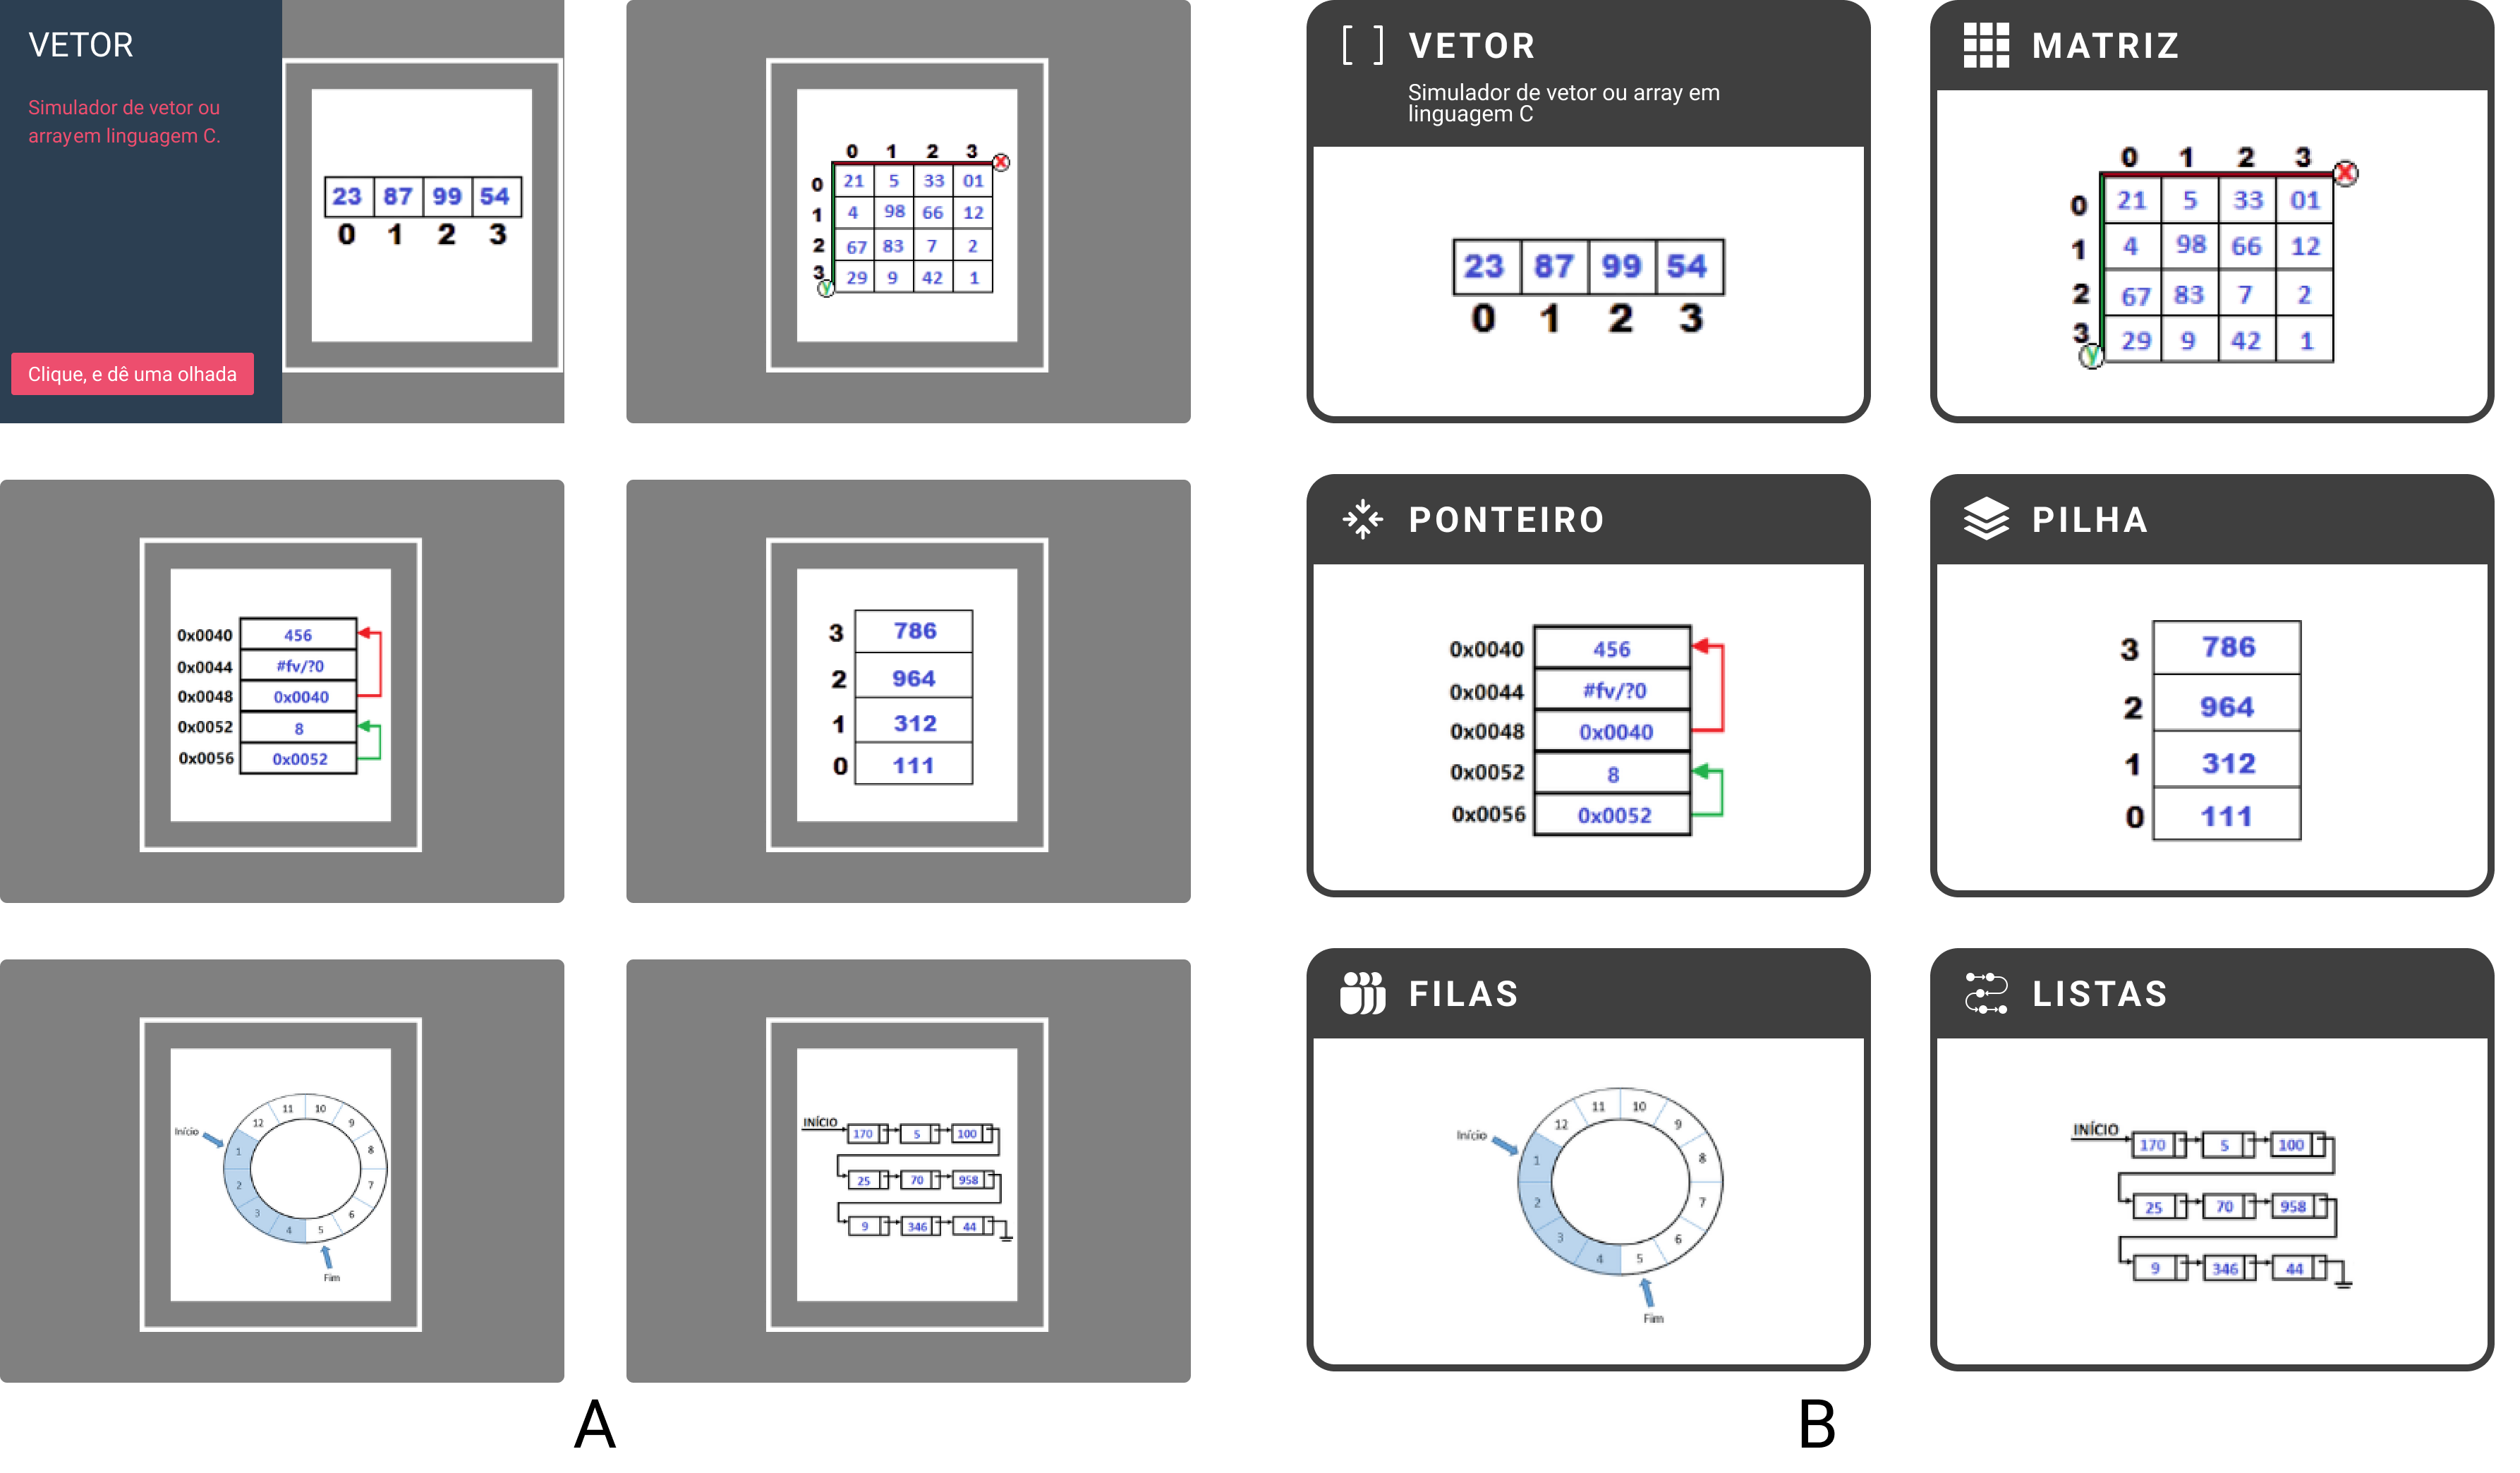
\includegraphics[scale=0.25]{figs/debugandoED-bloco-antes-depois-01.png}
	\end{center}
    \caption{\label{debugandoED-bloco-antes-depois-01}Exemplificação de Todos os Blocos: (A) Original; (B) Proposta.}
\end{figure}

%\newpage

\subsection{Campos de Entrada de Dados}
\label{Campos_de_Entrada_de_Dados}

Na \autoref{debugandoED-inputs}, pode-se notar que o sistema possui dois estilos diferentes de entrada de dados, logo não possui uma padronização nos \textit{inputs}.

Observando com mais cuidado, pode-se notar que várias heurísticas da \autoref{Heurísticas de Jakob Nielsen} são descumpridas, como: Consistência e padrões, Prevenção de erros, Estética e Design minimalista e Auxiliar usuários a reconhecer, diagnosticar e recuperar erros e no princípio da Proximidade da \autoref{Princípios de Gestalt}.


\begin{figure}[ht]
    \begin{center}
	    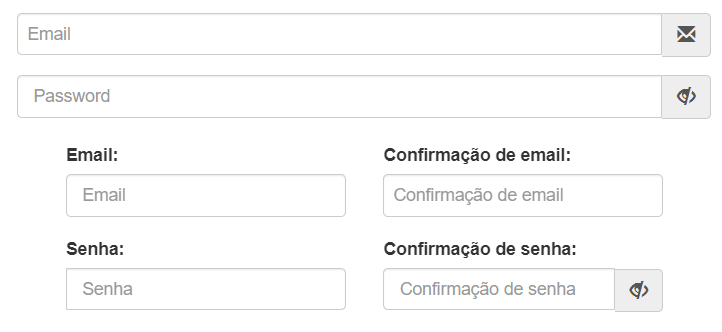
\includegraphics[scale=0.55]{figs/debugandoED-inputs.png}
	\end{center}
    \caption{\label{debugandoED-inputs}Campos de entrada atualmente na Plataforma.}
\end{figure}


Uma forma de resolver tais problemas, é na construção da identidade visual própria para os campos de entrada de dados, comumente os designers utilizam padrões e diretrizes já muito bem estabelecidos neste ramo, em suma a proposta aqui é basear-se na \autoref{Material_Design} que se trata do \textit{Material Design} (\autoref{debugandoED-inputs-md}).

\begin{figure}[ht]
    \begin{center}
	    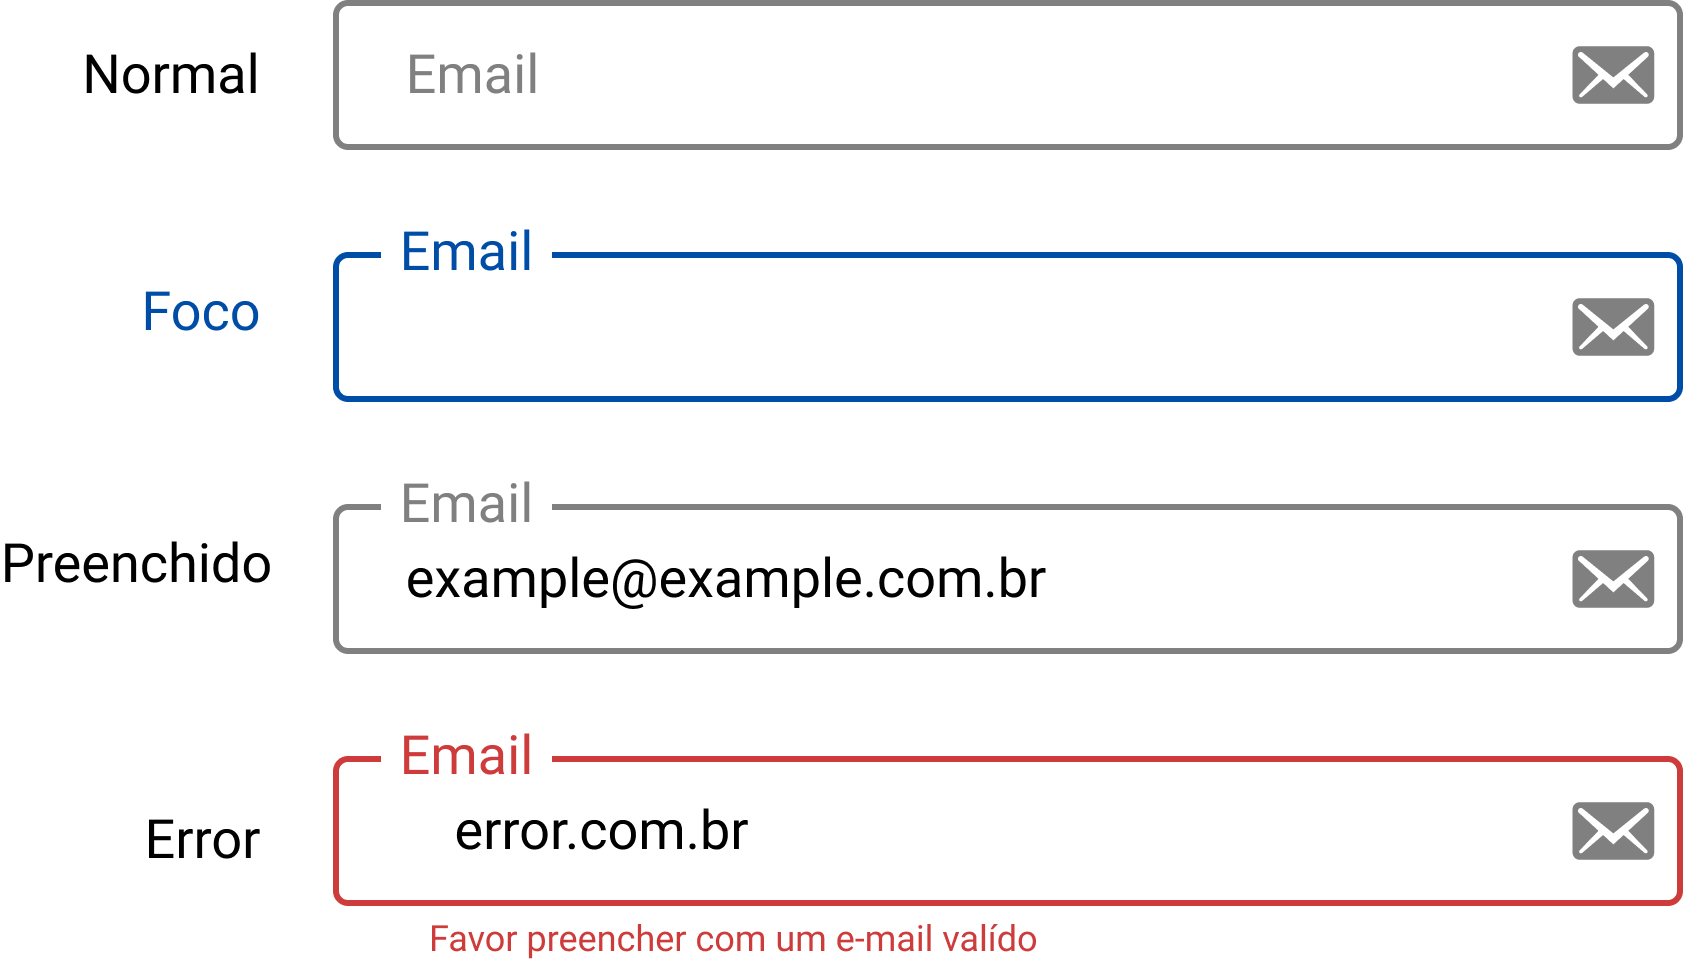
\includegraphics[scale=0.52]{figs/debugandoED-inputs-md.png}
	\end{center}
    \caption{\label{debugandoED-inputs-md}Exemplos de Campos de entrada - Baseados no \textit{Material Design}.}
\end{figure}

Pontos como Prevenção de erros e Auxiliar usuários a reconhecer, diagnosticar e recuperar erros, são muito bem tratados como é o exemplo \textbf{\textit{Error}} na \autoref{debugandoED-inputs-md}, como uma mudança visual na cor do \textit{input} e \textit{label}, como também uma mensagem auxiliando o usuário na correção do erro.

E os outros pontos citados no início desta seção, são resolvidos com a simplicidade e minimalismo no design empregado nestes campos, como o \textit{placeholder} simples. Este, que exibe o tipo do campo,  além do título para orientar o usuário durante o preenchimento.

\subsection{Formulário de Cadastro}
\label{Formulário de Cadastro}

Pensando-se na experiência do usuário, obviamente deve-se realizar uma pesquisa antes de qualquer tomada de decisão, mas pode-se notar na \autoref{debugandoED-form-antes-depois} - Antes, alguns pontos como: o campo de \texttt{Confirmação de email} e a seleção de \textbf{imagem para o perfil} aparentam ser desnecessários, a confirmação do endereço eletrônico pode ser verificada com o envio de um email solicitando uma verificação onde também aumenta a segurança garantindo que aquele endereço eletrônico utilizado no momento do cadastro é de fato do usuário, e a imagem para perfil é algo completamente desnecessário nesse momento, pois tal opção já existe na edição do perfil, sendo assim o formulário fica mais limpo.

Outro ponto é no campo de \textbf{Instituição de ensino}, onde é um \textit{input} do tipo de seleção, porém existem muitas opções para selecionar, podendo deixar alguns usuários perdidos, para melhorar tal campo a adição de digitar e filtrar entre essas opções traria uma grande melhora na experiência do usuário, maior ainda se fosse um campo auto completar.

O método citado acima pode ser utilizado em demais campos de seleção, como também transformar os campos de \textbf{Estado} e \textbf{Cidade} para seleção utilizando a \ac{API} de localidades\footnote{\url{https://servicodados.ibge.gov.br/api/docs/localidades}} do IBGE disponibilizada gratuitamente pra propósitos de se obter estados e cidades filtrados.

Devido aos princípios da Continuidade e do Ponto Focal da \autoref{Princípios de Gestalt}, nota-se a inversão dos botões e na suas respectivas estilizações na \autoref{debugandoED-form-antes-depois} (Depois), aumentando o foco e relevância no botão visualmente mais a direita cujo tem maior importância.

A demonstração dos pontos citados anteriormente pode ser visualizados na \autoref{debugandoED-form-antes-depois} (Depois).

\begin{figure}[htb]
    \begin{center}
	    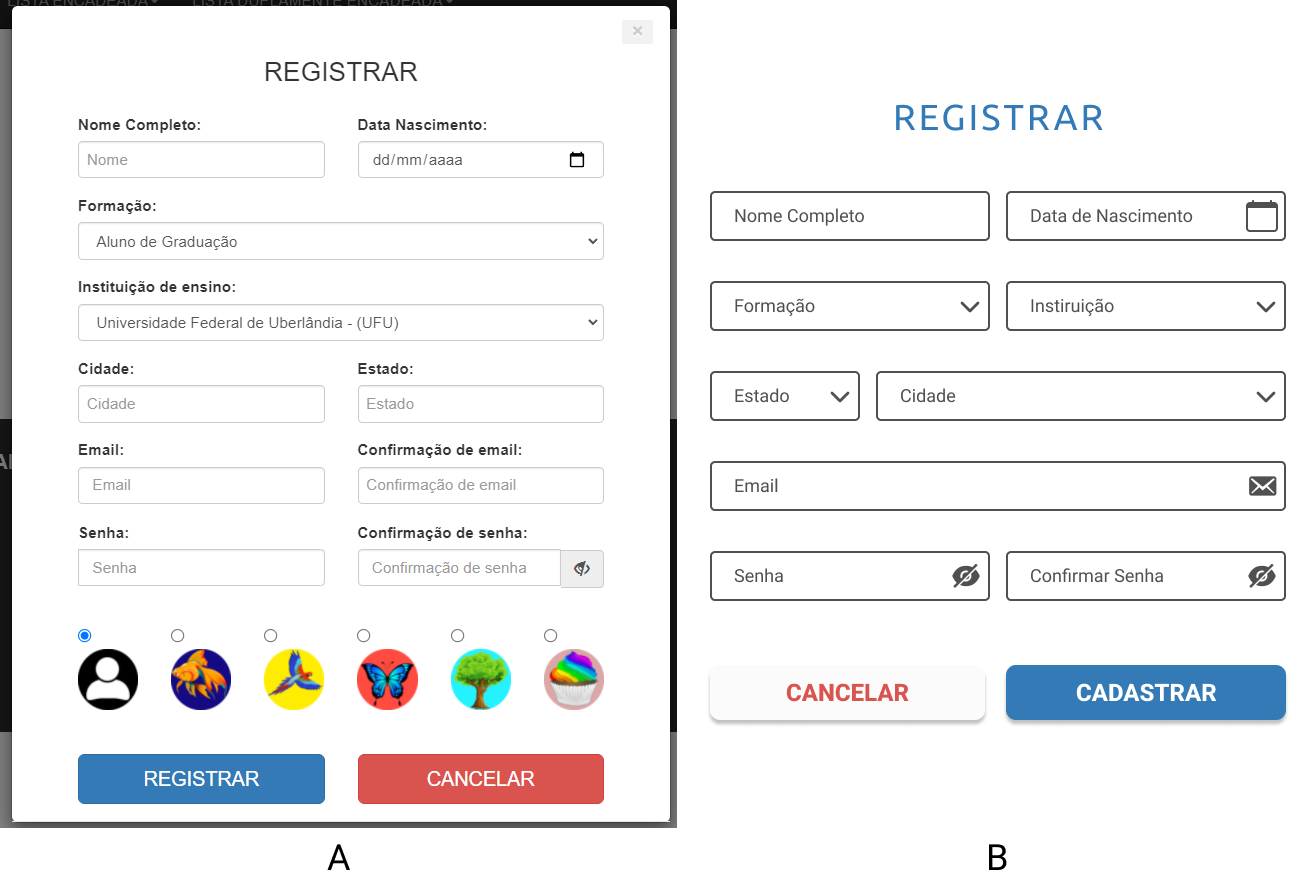
\includegraphics[scale=0.35]{figs/debugandoED-form-antes-depois.png}
	\end{center}
    \caption{\label{debugandoED-form-antes-depois}Formulário de Cadastro: (A) Original; (B) Proposta.}
\end{figure}

\subsection{Formulário de Login}
\label{Formulário de Login}

Como citado na \autoref{Formulário de Cadastro} os princípios da Continuidade e do Ponto Focal também são relevantes na \autoref{debugandoED-form-login-antes-depois}, devido a ter dois botões onde o mais a direita não possuiu maior importância neste fluxo, isto é contornado removendo o botão de cadastro e de forma sucinta substituído por um link, logo abaixo do botão Entrar.

Outro ponto relevante aqui é um pouco sugestivo, pois se trata do princípio da Região Comum da \autoref{Princípios de Gestalt}, onde facilmente é resolvido com alguns espaçamentos ou a simples remoção das linhas horizontais já empregaria tal espaçamento necessário.

\begin{figure}[htb]
    \begin{center}
	    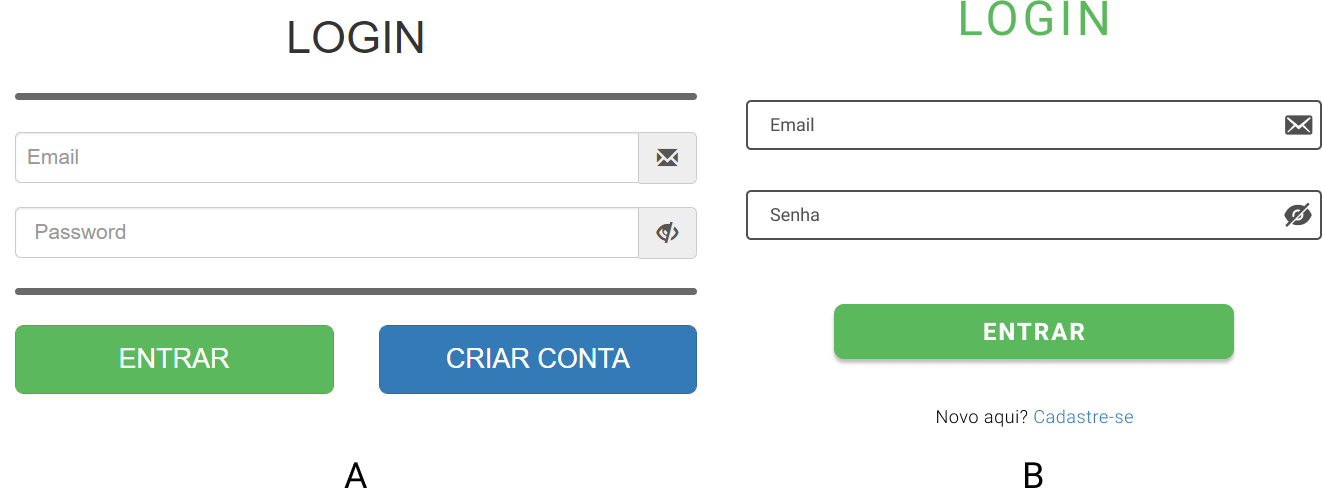
\includegraphics[scale=0.35]{figs/debugandoED-form-login-antes-depois.png}
	\end{center}
    \caption{\label{debugandoED-form-login-antes-depois}Formulário de Login: (A) Original; (B) Proposta.}
\end{figure}

\subsection{Conteúdo das Telas de Simulação}
\label{Conteúdo das Telas de Simulação}

As Figuras \ref{debugandoED-ponteiro-antes-01} e \ref{debugandoED-ponteiro-antes-02} são, respectivamente, capturas de tela do início e durante a simulação referente à execução de um ponteiro no contexto de programação.

\begin{figure}[htb]
    \begin{center}
	    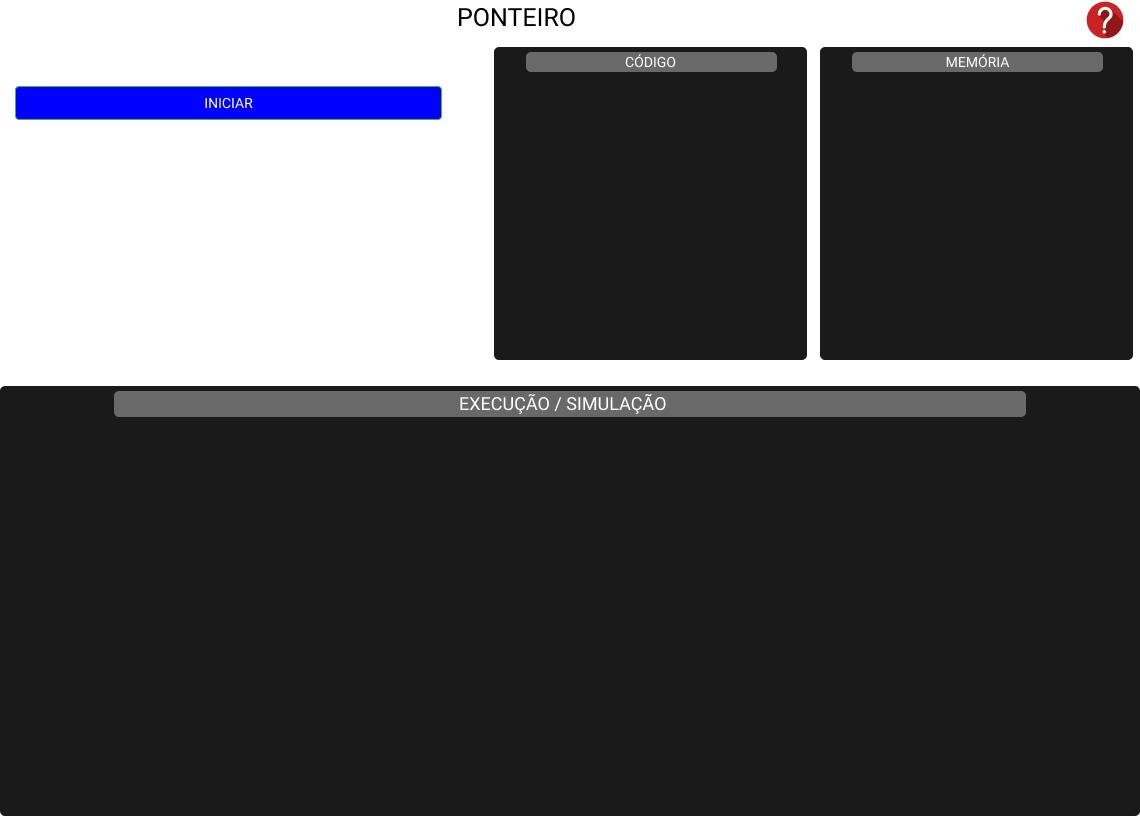
\includegraphics[scale=0.25]{figs/debugandoED-ponteiro-antes-01.png}
	\end{center}
    \caption{\label{debugandoED-ponteiro-antes-01}Simulação de Ponteiro - 1º Momento}
\end{figure}

Inicialmente na \autoref{debugandoED-ponteiro-antes-01}, nota-se apenas os quadros em fundo escuro, o que necessariamente não é um problema, mas sim uma identidade visual dependendo da comunicabilidade cujo desenvolvedor quer passar ao usuário final, porém, tais quadros também podem ser dispostos em uma tonalidade mais clara, obtendo um visual mais limpo com contraste não tão agressivos.

\begin{figure}[htb]
    \begin{center}
	    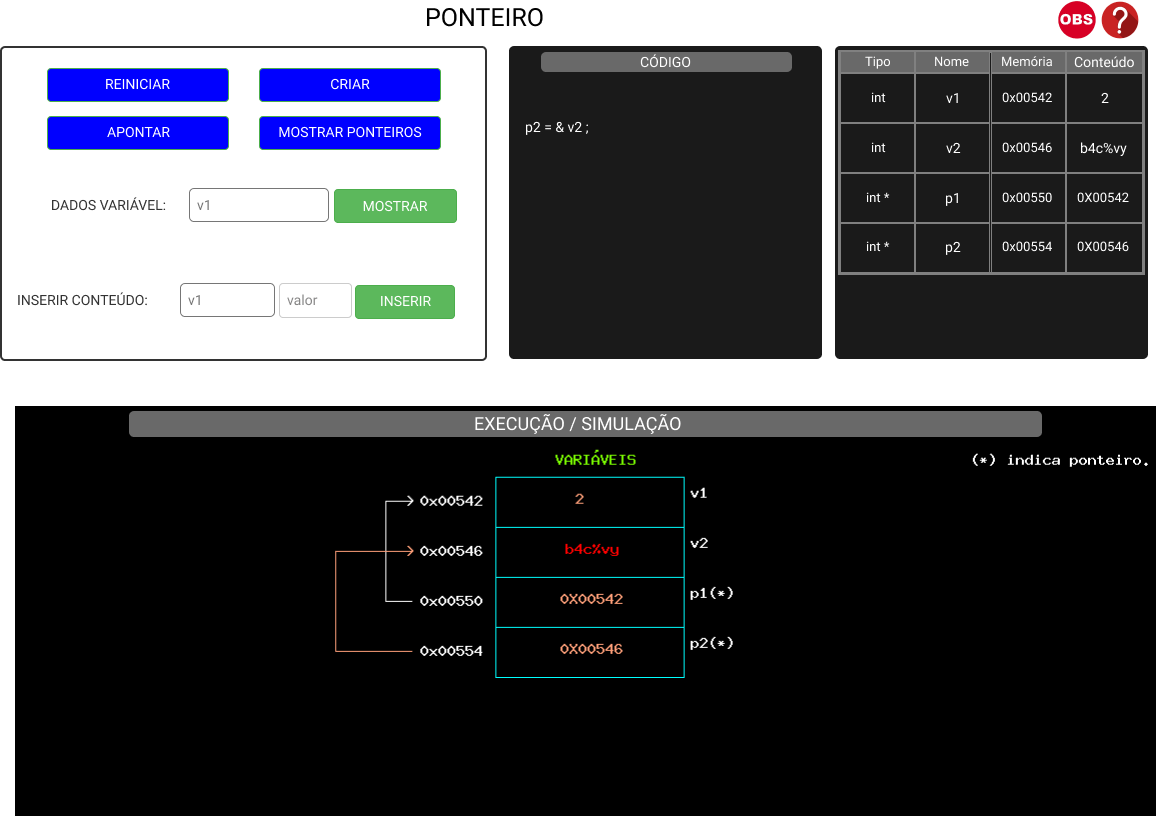
\includegraphics[scale=0.25]{figs/debugandoED-ponteiro-antes-02.png}
	\end{center}
    \caption{\label{debugandoED-ponteiro-antes-02}Simulação de Ponteiro - 2º Momento}
\end{figure}

\begin{figure}[htb]
    \begin{center}
	    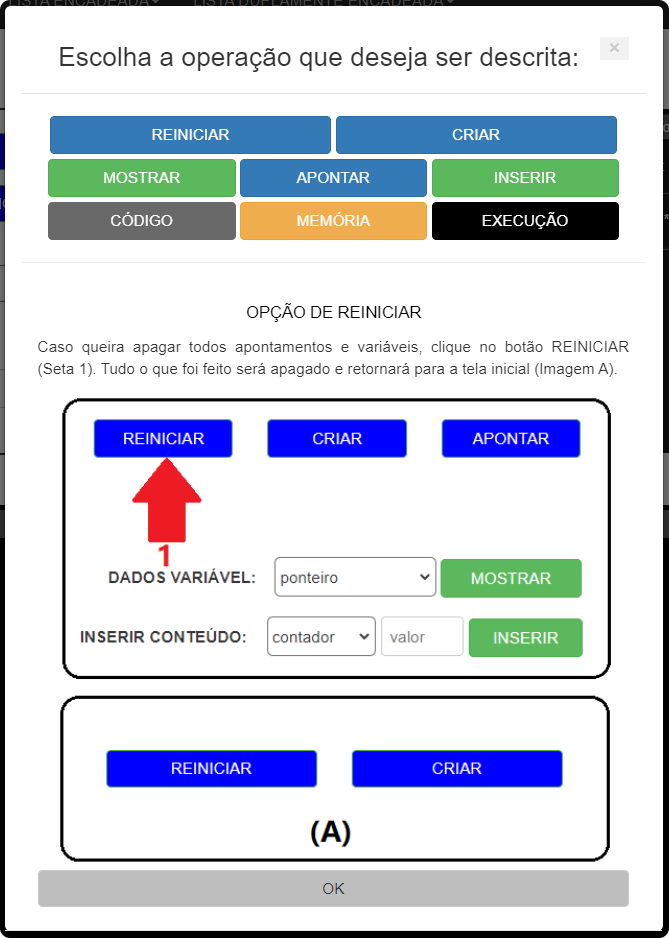
\includegraphics[scale=0.25]{figs/debugandoED-modais-help-01.png}
	\end{center}
    \caption{\label{debugandoED-modais-help-01}Modal de ajuda envolvidos na simulação de ponteiro}
\end{figure}

\begin{figure}[htb]
    \begin{center}
	    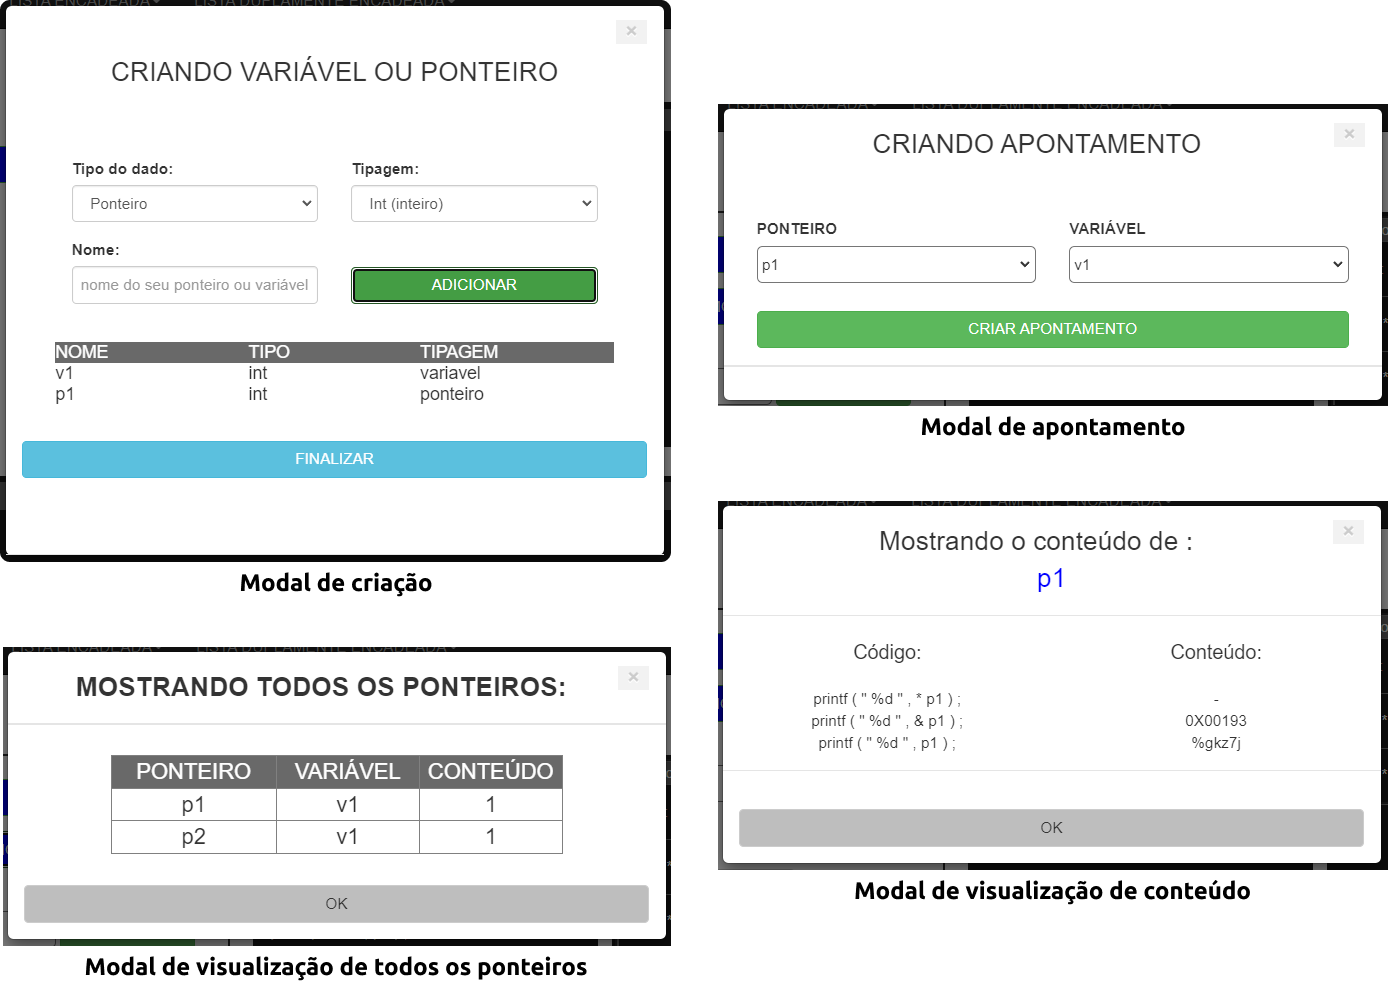
\includegraphics[scale=0.25]{figs/debugandoED-modais-antes-01.png}
	\end{center}
    \caption{\label{debugandoED-modais-antes-01}Modais envolvidos na simulação de ponteiro}
\end{figure}

A \autoref{debugandoED-ponteiro-antes-02}, nota-se que os quadros negros estão preenchidos com seus devidos conteúdos didáticos referente a uma simulação de ponteiro no contexto de programação, no mesmo pode-se notar, que o botão “Iniciar” deu lugar a um quadro com mais informações e ações para progredir na simulação, porém, de acordo com \autoref{Heurísticas de Jakob Nielsen}, algumas heurísticas não são totalmente exploradas corretamente, como:
\begin{itemize}
    \item A liberdade e controle do usuário, devido ao usuário ter que necessariamente realizar as ações da simulação através de modal (\autoref{debugandoED-modais-antes-01}) e devido a isso, caso precise consultar a documentação deverá fechar o modal e recomeçar.
    
    Pode-se observar na \autoref{debugandoED-modais-antes-01}, a falta consistência e padrões, como títulos em caixa alta e caixa baixa, em negrito e normal e falta de alinhamento em alguns elementos

    \item Reconhecer ao invés de lembrar é pouca explorada, pois, os botões possuem o mesmo padrão de cores, porém, com funções distintas, o que pode causar confusão no usuário na hora da utilização.

    \item Ajuda e documentação, até possui um modal dedicado a tais explicações para que o usuário não se percam na simulação. Porém, é muito densa a quantidade de informação em apenas um único local, outro ponto, é a falta de padronização nas cores dos botões dentro do modal como é mostrado na \autoref{debugandoED-modais-help-01} em relação aos botões reais no sistema.

\end{itemize}

As melhorias projetadas nas Figuras \ref{debugandoED-ponteiro-depois-01} e \ref{debugandoED-ponteiro-depois-02}, demonstra uma percepção no questionário realizado em termos de usabilidade e \ac{UX}. Obtendo uma evolução na comunicabilidade do simulador. O design da interface \ac{UI} foi refinado para promover uma interação mais intuitiva, alinhando-se com os princípios da \autoref{Princípios de Gestalt} para facilitar o reconhecimento de padrões.

\begin{figure}[htb]
    \begin{center}
        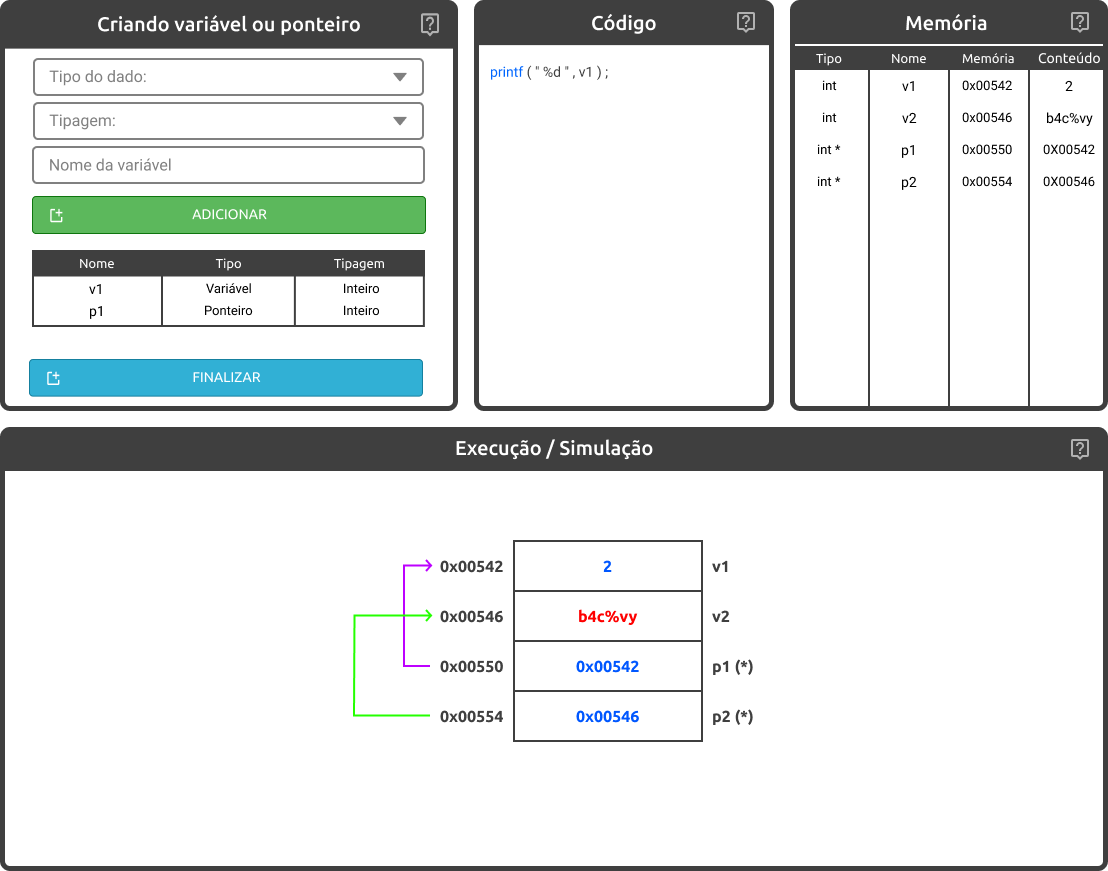
\includegraphics[scale=0.25]{figs/debugandoED-ponteiro-depois-01.png}
    \end{center}
    \caption{\label{debugandoED-ponteiro-depois-01}Simulação de Ponteiro - Melhorias Implementadas 01}
\end{figure}

\begin{figure}[htb]
    \begin{center}
        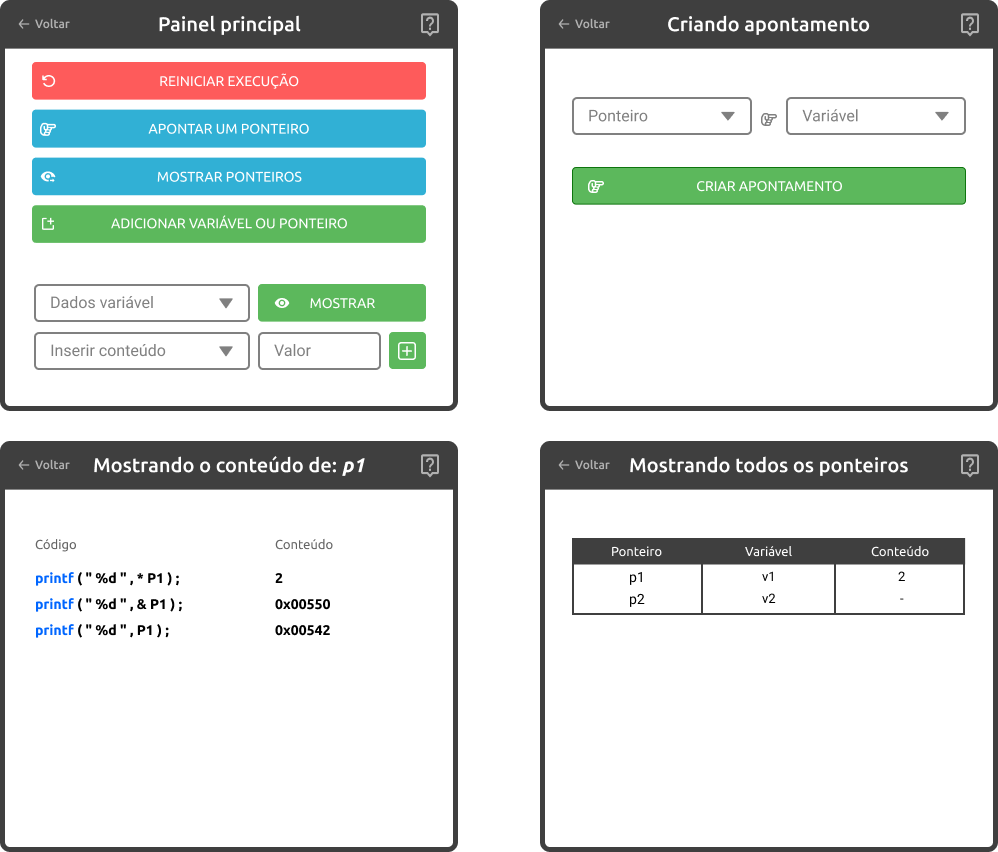
\includegraphics[scale=0.25]{figs/debugandoED-ponteiro-depois-02.png}
    \end{center}
    \caption{\label{debugandoED-ponteiro-depois-02}Simulação de Ponteiro - Melhorias Implementadas 02}
\end{figure}

Apresentando uma \ac{UI} aprimorada, com a utilização de esquemas de cores e tipografia para melhorar a legibilidade e a hierarquia visual, seguindo os princípios da \autoref{Princípios de Gestalt} para agrupamento e alinhamento. O design limpo e intuitivo promove uma experiência de usuário \ac{UX} positiva, em conformidade com as heurísticas de usabilidade da \autoref{Heurísticas de Jakob Nielsen}, particularmente no que diz respeito à consistência e padronização dos elementos de \ac{UI}.

A estrutura da informação e os elementos de navegação foram reorganizados para dar ao usuário maior controle e liberdade, permitindo uma exploração mais fluída e natural. Isso é evidente na inclusão de \textit{tooltips} e modais informativos, que são facilmente acessíveis sem interromper a tarefa do usuário, alinhando-se com o princípio de Ajuda e documentação das heurísticas de Nielsen.

Essas melhorias de interface não apenas aprimoram a estética, mas também reforçam a funcionalidade e a eficácia pedagógica da simulação, ao passo que a experiência de aprendizado se torna mais engajante e menos suscetível a erros de interpretação ou operação


%%%%%%%%%%%%%%%%%%%%%%%%%%%%%%%%%%%%%%%%%%%
%              Análises                   %
%%%%%%%%%%%%%%%%%%%%%%%%%%%%%%%%%%%%%%%%%%%

\section{Análise das Propostas por Experimento}

Esta seção apresentará as respostas obtidas nos questionários da pesquisa conduzida para este estudo. O objetivo principal é fornecer uma visão abrangente das percepções e opiniões coletadas por duas abordagens distintas: em relação à usabilidade e design e a experiência do usuário em interfaces da plataforma. As diferenças demográficas e de formação educacional entre esses dois grupos proporcionaram uma visão diversificada e enriquecedora das opiniões e perspectivas dos usuários. Foram conduzidos 2 experimentos: um voltado para estudantes e outro focado em profissionais. 

Para a realização dos experimentos, foi criado dois questionários para coletar dados sobre as percepções dos participantes em relação ao sistema DebugandoED\footnote{\url{https://debugandoed.facom.ufu.br/}} e suas respectivas telas propostas neste trabalho. Ambos os questionários compartilharam uma série de perguntas idênticas, com o propósito de avaliar as telas de login, cadastro, tela principal e tela de conteúdo. A distinção crítica entre os questionários ocorreu na primeira parte, na qual as perguntas demográficas e de conhecimento foram apresentadas aos participantes. Dentre as diversas questões, algumas delas baseiam-se na escolha entre telas (\autoref{fomuEscolha}), possibilitando a escolha da ``Imagem A'' (tela original da plataforma) ou ``Imagem B'' (proposta da mesma tela utilizando os conceitos/princípios).

\begin{figure}[ht]
    \begin{center}
	    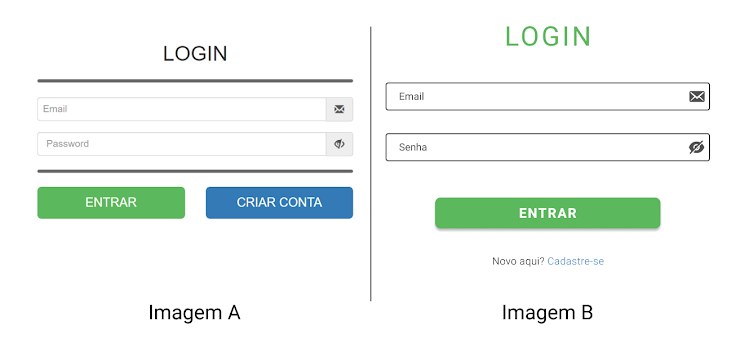
\includegraphics[scale=0.4]{figs/form_compara.png}
	\end{center}
    \caption{\label{fomuEscolha}Exemplo das imagens utilizadas nos questionários.}
\end{figure}

Todos os detalhes sobre os questionários, bem como todas as questões utilizadas, estão no \autoref{questionario_de_pesquisa}.

%A seção \ref{Pesquisa_de_Opinião_com_Estudantes}, concentra-se nas respostas e percepções compartilhados por um grupo representativo de estudantes universitários. Esses jovens representam a próxima geração de profissionais e pesquisadores nesta área de estudo. Suas opiniões e perspectivas podem oferecer uma visão valiosa sobre como a pesquisa e o conhecimento estão sendo percebidos pelos futuros atores do campo.

%A seção \ref{Pesquisa_de_Opinião_com_Profissionais}, concentra-se nas respostas e percepções coletadas junto a um grupo seleto de especialistas e profissionais da área. Esses participantes foram escolhidos por sua vasta experiência e conhecimento no domínio de estudo. Suas opiniões são fundamentais para oferecer uma perspectiva madura e experiente sobre as questões abordadas nesta pesquisa.

\subsection{Pesquisa de Opinião com Estudantes}
\label{Pesquisa_de_Opinião_com_Estudantes}

A pesquisa contou com a participação de um grupo diversificado de 33 respondentes, incluindo indivíduos de diferentes gêneros, faixas etárias, níveis de escolaridade e profissões, como ilustrado nas Figuras \ref{APB_01} e \ref{APB_02}. Os participantes variaram desde estudantes do ensino médio até aqueles com pós-doutorado e experiência em áreas como tecnologia, atendimento ao cliente, e ciências biológicas. Além disso, houve uma distribuição de níveis de experiência, com participantes desde juniores até sêniores em suas carreiras.

Além de suas características demográficas e educacionais, os participantes também foram questionados sobre seu conhecimento em \ac{UI} e \ac{UX}, \autoref{APB_03}, com algumas pessoas afirmando ter um entendimento desses conceitos, enquanto outras não estavam familiarizadas. No que diz respeito à \ac{UI}, 18 participantes afirmaram ter conhecimento, enquanto 15 declararam não estar familiarizados. Quanto à \ac{UX}, 13 participantes afirmaram ter conhecimento, enquanto 20 indicaram não estar familiarizados com o termo.

Esta diversidade de perfil dos participantes enriqueceu a pesquisa, fornecendo uma variedade de perspectivas e experiências que contribuíram para uma análise abrangente das telas de interface do usuário e da experiência do usuário. 

Além disso, é importante destacar que o \autoref{respostas_dos_estudantes} contém capturas de tela detalhadas exclusivamente das respostas do grupo de estudantes, proporcionando uma visão mais aprofundada das percepções dessa parcela específica de participantes na pesquisa.

Após a análise e avaliação das respostas dos participantes, tem-se: 

%A seguir, apresentaremos as conclusões e \textit{insights} obtidos com base nas respostas e avaliações desses participantes.

\begin{itemize}
    \item \textbf{Análise das Telas de Login}
    
    Durante esta pesquisa, foram avaliadas as telas de login em vários aspectos de usabilidade e design. Os resultados revelaram uma clara preferência pela ``Imagem B'' em categorias cruciais, como \textit{layout} atrativo, experiência intuitiva, organização de informações clara e distribuição eficiente de campos de entrada. No entanto, a ``Imagem A'' recebeu elogios por sua mensagem de erro e rótulos de botões informativos. Alguns participantes sugeriram combinar as duas telas, destacando pontos fortes de cada uma. Em resumo, enquanto a ``Imagem B'' se destacou como a escolha preferida na maioria das categorias, a ``Imagem A'' demonstrou pontos fortes específicos que merecem consideração na otimização da experiência do usuário.
    
    \item \textbf{Análise das Telas de Cadastro}
    
    Na análise comparativa para a tela de cadastro, observou-se uma preferência geral pelos elementos da ``Imagem B'' em diversas categorias, incluindo \textit{layout}, organização, distribuição de campos de entrada, mensagens de erro e conteúdo textual. A ``Imagem A'' recebeu elogios por sua estética visual, enquanto a ``Imagem B'' se destacou por oferecer uma experiência mais intuitiva e funcional. As sugestões apontaram para a possibilidade de combinar as forças de ambas as imagens, aproveitando a estética da ``Imagem A'' com a funcionalidade da ``Imagem B'', ressaltando a importância de equilibrar forma e função na criação de interfaces de usuário.
    
    \item \textbf{Análise da Tela Principal}
    
    Na avaliação para a tela principal, a preferência geral recai sobre a ``Imagem B'' em uma série de aspectos, incluindo o \textit{layout} atrativo, abordagem objetiva na disposição de elementos, experiência de uso confortável, organização eficiente de informações, distribuição equilibrada de elementos e clareza nos blocos de conteúdo. A ``Imagem A'' foi elogiada apenas por sua estética visual em algumas respostas. A sugestão apontada é a de que a ``Imagem B'' poderia ser aprimorada com cores mais claras nos elementos do corpo da página, semelhantes à ``Imagem A''. A predominância da preferência pela ``Imagem B'' sugere uma abordagem mais funcional e eficaz na criação da tela principal.
    
    \item \textbf{Análise da Tela de Conteúdo}
    
    Na avaliação para a tela de conteúdo, a preferência geral recai sobre a ``Imagem B'' em diversos aspectos, incluindo o layout atrativo, abordagem objetiva na disposição e organização dos blocos de conteúdo, experiência de uso confortável, organização eficiente de informações e distribuição equilibrada de elementos. A sugestão apontada é a de que a ``Imagem B'' poderia incorporar um modo escuro (\textit{dark mode}) para maior conforto visual, especialmente ao exibir código na tela. A predominância da preferência pela ``Imagem B'' sugere que sua abordagem é mais eficaz e intuitiva para a apresentação de conteúdo.
\end{itemize}

Em suma, os resultados da análise das telas de login, cadastro, tela principal e tela de conteúdo revelaram uma tendência clara em favor da ``Imagem B'' por parte dos estudantes que participaram do questionário. Essa preferência foi fundamentada em vários aspectos, como \textit{layout} atrativo, organização intuitiva, distribuição eficiente de informações e mensagens de erro adequadas. No entanto, é importante notar que a ``Imagem A'' também recebeu elogios por sua estética visual e pela presença de \textit{labels} no formulário, que foram considerados benéficos para usuários com mais idade.

As sugestões dos participantes apontaram para a possibilidade de combinar elementos positivos de ambas as imagens, destacando a importância de equilibrar forma e função na criação de interfaces de usuário. Além disso, houve recomendações para melhorias específicas, como a incorporação de um modo escuro na ``Imagem B'' para melhorar o conforto visual durante a visualização de código.

Em última análise, os resultados enfatizam a importância de considerar as preferências e necessidades dos usuários ao projetar interfaces, buscando o equilíbrio entre estética e funcionalidade para proporcionar uma experiência de usuário superior.


\subsection{Pesquisa de Opinião com Profissionais}
\label{Pesquisa_de_Opinião_com_Profissionais}

A pesquisa foi conduzida com um grupo de participantes que demonstram uma forte ligação com o campo do desenvolvimento de software e áreas relacionadas. Estes respondentes apresentam uma variedade de perfis, incluindo diferentes faixas etárias e níveis de escolaridade, com muitos deles possuindo graduações e especializações.

A maioria dos participantes está atualmente trabalhando com desenvolvimento de software ou funções semelhantes, ocupando cargos que variam de estagiários a profissionais sêniores. Suas profissões abrangem várias áreas, como desenvolvedores \textit{full stack}, engenheiros de software, programadores, entre outros. Essa diversidade de cargos e níveis de experiência contribui para uma visão abrangente das perspectivas dos profissionais de desenvolvimento.

Além disso, a pesquisa contou com 11 profissionais, cujas informações demográficas estão detalhadas nas Figuras \ref{APC_01}, \ref{APC_02} e \ref{APC_03}. Destaca-se que apenas 1 participante deste grupo indicou não ter familiaridade com os conceitos de \ac{UI} e \ac{UX}. O conhecimento específico desses profissionais em \ac{UI} e \ac{UX} pode ser encontrado na \autoref{APC_03}. Todas as respostas desse grupo estão compiladas no \autoref{respostas_dos_profissionais}, que consiste em capturas de tela detalhadas das respostas fornecidas por cada profissional participante da pesquisa.

A partir dessas informações, foi possível esperar que as respostas e avaliações dos participantes forneçam \textit{insights} valiosos sobre as telas de interface do usuário e a experiência do usuário, com base em suas experiências e conhecimentos especializados. Essa perspectiva especializada é fundamental para uma análise aprofundada da pesquisa em questão. 

Após a análise e avaliação das respostas dos participantes, tem-se: 

\begin{itemize}
    \item \textbf{Análise da Tela de Login}
    
    Durante a pesquisa, ao se comparar as duas telas de login, nota-se uma clara preferência pela ``Imagem B'' entre os participantes. Esta foi considerada mais atrativa, intuitiva e com uma organização de informações superior. Além disso, a ``Imagem B'' se destacou por possuir uma distribuição mais eficiente dos campos de entrada e mensagens de erro adequadas. Apesar de algumas críticas pontuais à ``Imagem A'', como a presença de elementos visuais excessivos e possíveis problemas de legibilidade, a maioria dos participantes concordou que a ``Imagem B'' é a opção mais objetiva e eficaz para fazer login.
    
    \item \textbf{Análise da Tela de Cadastro}
    
    As telas de cadastro também foram avaliadas, e novamente, a ``Imagem B'' se destacou. Esta foi consistentemente elogiada por sua organização, intuitividade e mensagens de erro adequadas. Por outro lado, a ``Imagem A'' muitas vezes foi vista como sobrecarregada de informações ou elementos visuais excessivos. Por outro lado, um ponto positivo da ``Imagem A'' foi a presença de \textit{labels} no formulário, que os participantes consideraram úteis, especialmente para os usuários com mais idade. Portanto, este estudo indica a preferência pela ``Imagem B'' para fins de cadastro, mas também ressalta a importância de considerar características específicas, como os \textit{labels}, para melhorar a experiência do usuário.
    
    \item \textbf{Análise da Tela Principal}
    
    Ao avaliar a tela da página principal, a ``Imagem B'' se destacou em aspectos cruciais, como \textit{layout}, organização e funcionalidade. Esta foi consistentemente escolhida pelos participantes como a mais eficaz em proporcionar uma experiência de usuário intuitiva e visualmente agradável. Embora a ``Imagem A'' tenha recebido algumas críticas, como a presença de informações excessivas, ainda foi elogiada por sua navegação em alguns casos. Em resumo, os resultados indicam uma clara preferência dos participantes pela ``Imagem B'' em design e usabilidade.

    \item \textbf{Análise da Tela de Conteúdo}
    
    Ao analisar as respostas sobre a a tela de conteúdo, percebe-se que a maioria preferiu a ``Imagem B'' em design atrativo, organização, interatividade e consistência textual. A ``Imagem B'' se destacou principalmente por sua abordagem objetiva, distribuição equilibrada de elementos e eficiência na apresentação das informações. Por outro lado, a ``Imagem A'' foi ocasionalmente apontada como tendo excesso de informações ou elementos visuais, o que pode prejudicar a experiência do usuário. Em resumo, a maioria dos participantes identificou a ``Imagem B'' como a opção mais adequada para proporcionar uma experiência de usuário superior na apresentação de conteúdo.
    
\end{itemize}

Em síntese, a análise abrangente das quatro áreas distintas, com base nas respostas de profissionais da área, revelou uma clara preferência pela ``Imagem B'' em quase todos os aspectos avaliados. Essa preferência foi fundamentada na atratividade visual, intuição, organização eficaz de informações e distribuição eficiente de elementos.

Apesar disso, a ``Imagem A'' não deve ser ignorada, pois, demonstrou méritos específicos, como a presença de \textit{labels} úteis para facilitar a experiência de usuários com mais idade. Portanto, a pesquisa indica a ``Imagem B'' como a escolha preferencial para a tela de login, cadastro, tela principal e tela de conteúdo. No entanto, destaca-se a importância de avaliar cuidadosamente as características específicas de cada imagem, aproveitando os pontos fortes de ambas, para otimizar a experiência do usuário de maneira global e eficaz.
